% \documentclass[12pt]{article}
\documentclass[BCOR=0mm,DIV11,titlepage,a4paper,oneside]{scrbook}
\usepackage{scrhack}
\usepackage[ngerman]{babel}
\usepackage[utf8x]{inputenc}
\usepackage{amsmath}
\usepackage{graphicx}
\usepackage{caption}
\usepackage[colorinlistoftodos]{todonotes}
\usepackage{subcaption}

%fancyheadings funktioniert nicht mehr mit der KOMA Script Klasse scrbook

\usepackage{wrapfig}

\usepackage[authoryear,round]{natbib}
\usepackage{usebib}
\bibinput{literatur}

% Mittels [H] können Bilder genau an einer Stelle positioniert werden
\usepackage{float}

\usepackage[breaklinks]{hyperref}

% bewirkt das HyperLinks in der PDF nicht umrandet oder farbig sind
\hypersetup{colorlinks=false}

% package for colored text
% black,white,green,red,blue,yellow,cyan,magenta
\usepackage{color}

% package for colored tables
\usepackage{colortbl}

%Paket zur Erzeugung von Anführungszeichen durch \enquote{Text}
\usepackage[ngerman]{babel}
\usepackage[babel, german=quotes]{csquotes}

%Verhindern, dass eine neue Seite für ein einzelnes Wort/Zeile verwendet wird
\clubpenalty = 10000 % schliesst Schusterjungen aus 
\widowpenalty = 10000 % schliesst Hurenkinder aus (keine Beleidigung, sondern wirklich ein Fachbegriff)

\usepackage{lipsum}

% LISTINGS Code Highlighting Setup START
\usepackage{upquote}
\usepackage{listings}
\definecolor{editorGray}{rgb}{0.95, 0.95, 0.95}
\definecolor{editorOcher}{rgb}{1, 0.5, 0} % #FF7F00 -> rgb(239, 169, 0)
\definecolor{editorGreen}{rgb}{0, 0.5, 0} % #007C00 -> rgb(0, 124, 0)
\definecolor{airforceblue}{rgb}{0.36, 0.54, 0.66}

% \lstdefinelanguage{JavaScript}{
%   morekeywords={typeof, new, true, false, catch, function, return, null, catch, switch, var, if, in, while, do, else, case, break},
%   morecomment=[s]{/*}{*/},
%   morecomment=[l]//,
%   morestring=[b]",
%   morestring=[b]'
% }

\lstdefinelanguage{JavaScript}{
  keywords={typeof, new, true, false, catch, function, return, null, catch, switch, var, if, in, while, do, else, case, break},
  keywordstyle=\color{blue}\bfseries,
  ndkeywords={class, export, boolean, throw, implements, import, this},
  ndkeywordstyle=\color{airforceblue} \bfseries,
  identifierstyle=\color{black},
  sensitive=false,
  comment=[l]{//},
  morecomment=[s]{/*}{*/},
  commentstyle=\color{purple}\ttfamily,
  stringstyle=\color{red}\ttfamily,
  morestring=[b]',
  morestring=[b]"
}

\lstdefinelanguage{HTML5}{
  language=html,
  sensitive=true, 
  alsoletter={<>=-},
  otherkeywords={
  % HTML tags
  <html>, <head>, <template>, </template>, <template, <section, </section>, <header, </header>, <ul, </ul>, <li, </li>, <title>, </title>, <div>, </div>, <meta, />, </head>, <body>,
  <canvas, \/canvas>, <script>, </script>, </body>, </html>, <nav>, </nav>, <!, html>, <style, </style>, ><
  },  
  ndkeywords={
  % General
  =,
  % HTML attributes
  charset=, id=, width=, height=, class=, lang=, v-for=,
  % CSS properties
  border:, transform:, -moz-transform:, transition-duration:, transition-property:, transition-timing-function:
  },  
  morecomment=[s]{<!--}{-->},
  tag=[s]
}

\lstset{
  % Basic design
  backgroundcolor=\color{editorGray},
  basicstyle={\small\ttfamily},   
  frame=l,
  % Line numbers
  xleftmargin={0.75cm},
  numbers=left,
  stepnumber=1,
  firstnumber=1,
  numberfirstline=true,
  % Code design   
  keywordstyle=\color{blue}\bfseries,
  commentstyle=\color{darkgray}\ttfamily,
  ndkeywordstyle=\color{editorGreen}\bfseries,
  stringstyle=\color{editorOcher},
  % Code
  language=HTML5,
  alsolanguage=JavaScript,
  alsodigit={.:;},
  tabsize=2,
  showtabs=false,
  showspaces=false,
  showstringspaces=false,
  extendedchars=true,
  breaklines=true,        
  % Support for German umlauts
  literate=%
  {Ö}{{\"O}}1
  {Ä}{{\"A}}1
  {Ü}{{\"U}}1
  {ß}{{\ss}}1
  {ü}{{\"u}}1
  {ä}{{\"a}}1
  {ö}{{\"o}}1
}

\lstset{literate=
  {á}{{\'a}}1 {é}{{\'e}}1 {í}{{\'i}}1 {ó}{{\'o}}1 {ú}{{\'u}}1
  {Á}{{\'A}}1 {É}{{\'E}}1 {Í}{{\'I}}1 {Ó}{{\'O}}1 {Ú}{{\'U}}1
  {à}{{\`a}}1 {è}{{\`e}}1 {ì}{{\`i}}1 {ò}{{\`o}}1 {ù}{{\`u}}1
  {À}{{\`A}}1 {È}{{\'E}}1 {Ì}{{\`I}}1 {Ò}{{\`O}}1 {Ù}{{\`U}}1
  {ä}{{\"a}}1 {ë}{{\"e}}1 {ï}{{\"i}}1 {ö}{{\"o}}1 {ü}{{\"u}}1
  {Ä}{{\"A}}1 {Ë}{{\"E}}1 {Ï}{{\"I}}1 {Ö}{{\"O}}1 {Ü}{{\"U}}1
  {â}{{\^a}}1 {ê}{{\^e}}1 {î}{{\^i}}1 {ô}{{\^o}}1 {û}{{\^u}}1
  {Â}{{\^A}}1 {Ê}{{\^E}}1 {Î}{{\^I}}1 {Ô}{{\^O}}1 {Û}{{\^U}}1
  {Ã}{{\~A}}1 {ã}{{\~a}}1 {Õ}{{\~O}}1 {õ}{{\~o}}1
  {œ}{{\oe}}1 {Œ}{{\OE}}1 {æ}{{\ae}}1 {Æ}{{\AE}}1 {ß}{{\ss}}1
  {ű}{{\H{u}}}1 {Ű}{{\H{U}}}1 {ő}{{\H{o}}}1 {Ő}{{\H{O}}}1
  {ç}{{\c c}}1 {Ç}{{\c C}}1 {ø}{{\o}}1 {å}{{\r a}}1 {Å}{{\r A}}1
  {€}{{\euro}}1 {£}{{\pounds}}1 {«}{{\guillemotleft}}1
  {»}{{\guillemotright}}1 {ñ}{{\~n}}1 {Ñ}{{\~N}}1 {¿}{{?`}}1
}
\renewcommand{\lstlistingname}{Codebeispiel}% Listing -> Algorithm
\renewcommand{\lstlistlistingname}{Codeverzeichnis}% List of Listings -> List of Algorithms

% LISTINGS Code Highlighting Setup END

\setlength{\parskip}{0.7em}

\begin{document}

%!TEX root = ../main.tex
\begin{titlepage}

\begin{center}

% Logo der Technische Hochschule Köln
% Kann auch in dieser Form in Schwarz/Weiß ausgedruckt werden; Graustufen sollten der .tif Version entsprechen
\begin{figure}[!ht]
%	\centering
		
\includegraphics[width=0.26\textwidth]{images/THlogoheader.pdf}
\end{figure}

\vspace{1.5cm}

%Deutscher Titel
\begin{rmfamily}
\begin{huge}
\textbf{ Erstellung einer isolierten Vue-Komponenten Bibliothek im Zusammenspiel mit dem Utility-Class-Framework Tailwindcss}\\	
\end{huge}
\vspace{0.5cm}
\begin{LARGE}
Entwicklung und Dokumentation anpassbarer Vue-Komponenten für kontinuierlich wachsende Webplattformen am Beispiel einer instanzierbaren Plattformlösung der AVACO GmbH. \\
\end{LARGE}
\end{rmfamily}

\vspace{0.8cm}

%Englischer Titel
% \begin{rmfamily}
% \textbf{\LARGE Title in English}\\
% \large with a very\\long subtitle\\
% \normalsize
% \end{rmfamily}

% \vspace{1.2cm}

%Bachelorarbeit 
\begin{LARGE}
\begin{scshape}
Exposé zum Praxisprojekt\\[0.8em]
\end{scshape}
\end{LARGE}

%ausgearbeitet von...
\begin{large}
ausgearbeitet von\\ 
\vspace{0.3cm}
\begin{LARGE}
Marvin Christian Klimm\\
\end{LARGE}
\end{large}

\vspace{1.2cm}

\vspace{0.6cm}

%vorgelegt an der...
\begin{large}
vorgelegt an der\\ 
\vspace{0.2cm}
\begin{scshape}
Technischen Hochschule Köln\\
Campus Gummersbach\\
Fakultät für Informatik und\\
Ingenieurwissenschaften\\
\end{scshape}
\end{large}

\vspace{0.6cm}

%im Studiengang...
\begin{large}
im Studiengang\\ 
\vspace{0.1cm}
\textsc{Medieninformatik}
\end{large}


\vspace{1.1cm}

%Autor der Bachelorarbeit und die Prüfer
\begin{tabular}{rl}
      Hochschul-Betreuer:  &  Prof. Christian Noss\\
       					&  \small Technische Hochschule Köln \\[1.0em]
      Unternehmensansprechpartner:  &  Thomas Brambring\\
       					&  \small AVACO GmbH\\
\end{tabular}

\vspace{0.7cm}

%Ort, Monat der Abgabe
\begin{large}
Gummersbach, im August \the\year
\end{large}

\end{center}

\newpage
\thispagestyle{empty}

%Kontaktmöglichkeiten des Autors und der Prüfer
\begin{center}
\begin{tabular}{rl}
							&  \\[20.0em]
							
\large \textbf{Adressen:}	& \quad Marvin Christian Klimm\\
							& \quad Am Hepel 61\\
							&	\quad 51643 Gummersbach\\
							& \quad studies@marvinklimm.de\\[2.0em]
							
							& \quad Prof. Christian Noss\\
							& \quad Technische Hochschule Köln\\
							& \quad Institut für Informatik\\
							&	\quad Steinmüllerallee 1\\
							&	\quad 51643 Gummersbach\\
							& \quad christian.noss@th-koeln.de\\[2.0em]
							
							& \quad Thomas Brambring\\
							& \quad AVACO GmbH\\
							&	\quad Löhestraße 18\\
							&	\quad 53773 Hennef (Sieg)\\
							& \quad t.brambring@avaco.io\\[2.0em]
\end{tabular}
\end{center}

\end{titlepage}


\chapter*{Vorbemerkung}
\label{sec:vorbemerkung}

Diese Arbeit wurde im Rahmen eines Firmenprojekte angefertigt und dokumentiert die Probleme, Anforderungen, Herangehensweisen und Lösungen die während der Bearbeitung herausgestellt wurden. Das Endprodukt, eine Komponentenbibliothek, dieser Arbeit ist Eigentum der AVACO GmbH und wurde noch vor Anfertigung dieses Dokumentes fertiggestellt.

Die Ideen, Grundkonzepte sowie die Codebasis wurden jedoch vor und während der Bearbeitung des Firmenprojektes in einem persönlichen Freizeitprojekt erarbeitet und parallel zur Anfertigung dieser Dokumentation in einem freien Projekt nochmals angewandt.

Der Referenzcode dieses Projektes kann unter folgenden URLs aufgerufen werden:
\begin{itemize}
  \item \textbf{Vollständiges Referenzrepository}\newline
  \url{https://github.com/netzfluencer/tailwindstories}

  \item \textbf{Version mit Storybook Setup}\newline
  \url{https://github.com/netzfluencer/tailwindstories/releases/tag/v0.1.1-alpha}

  \item \textbf{Version mit Tailwindcss Setup}\newline
  \url{https://github.com/netzfluencer/tailwindstories/releases/tag/v0.2.0-alpha}

  % \item \textbf{Bibliothek mit Beispielkomponenten} (Branch: \textit{example})\newline
  % \url{https://github.com/netzfluencer/tailwindstories/tree/example}
\end{itemize}


\tableofcontents
\setcounter{page}{1}
\newpage

\chapter{Einleitung}
\label{cha:Einleitung}

\begin{quotation}
	\emph{``While the utility-class-focused approach of new frameworks like Tailwind CSS make you question everything you know about writing “proper” semantic CSS, its 81\% satisfaction ratio means that it might be time to reconsider our old preconceived notions…''}
	\citep{StateCSS2019_Frameworks}
\end{quotation}

In der aktuellen Studie \textit{The State of CSS 2019} haben Raphaël Benitte und Sacha Greif herausgestellt, dass das neuartige Utility-Frist CSS-Framework \textit{Tailwind CSS} neben allen anderen verglichenen Frameworks die höchste Entwicklerzufriedenheit verzeichnen konnte.

Seit 2017 entwickelt die AVACO GmbH das anpassbare Webportal \textit{My.PORTAL}, das als Handels-, Kommunikations- und Kollaborationslösung in unterschiedlichen Nutzungskontexten eingesetzt werden kann. Dabei dienten bisher das Framework Bootstrap und der CSS-Preprozessor \textit{Syntactically Awesome Style Sheets} (i.F. SASS) als Hauptwerkzeuge für das Styling der wachsenden Vue-Applikation. Mit dem kontinuierlichen Wachstum begegnete das Frontend-Team neuen Herausforderungen in der Frontendentwicklung und insbesondere in der Gestaltung von wiederverwendbaren Vue-Komponenten sowie Style-Elementen. Diese Herausforderungen sind insbesondere in den Bereichen des Komponentenmanagements, der Komponentenentwicklung und des Komponentenstylings zu identifizieren und sollen nun, durch die Einführung einer neuen Komponentenbibliothek sowie Tailwind CSS und PostCSS als neue Gestaltungsbasis, gelöst werden.

Diese Arbeit befasst sich mit der Erstellung der neuen Vue-Komponenten-Bibliothek und der Einführung von Tailwind CSS im Frontend der aktuellen Vue-Applikation.
Dabei sollen Komponenten aus der Bibliothek isoliert bzw. unabhängig vom Hauptprojekt entwickelt, gestaltet und wiederverwendet werden können. Langfristig soll die neue Komponentenbibliothek fähig sein die bereits existierende Komponentenbibliothek zu ersetzten.

Dazu sollen zunächst die Herausforderungen und Probleme in der aktuellen Frontendarbeit von \textit{My.PORTAL} herausgestellt werden. Anschließend erfolgt eine Ermittlung der Anforderungen an die neue Komponentenbibliothek auf dessen Grundlage ein passendes Framework ausgewählt werden soll. Desweiteren sollen die Chancen und Risiken die mit der Einführung von Tailwind CSS verbunden sind ermittelt werden um dann schließlich Tailwind CSS im gesamten Frontend einzuführen.

Anschließend erfolgt eine Bewertung der Implementierung anhand aller vorher herausgestellten Herausforderungen, Anforderungen, Chancen und Risiken. Neue Herausforderungen, Chancen und Risiken werden dargelegt um schließlich auch einen Ausblick auf die neue Vue Version 3 in Bezug auf diese Arbeit anfertigen zu können.
\chapter{Kontext der Arbeit}
\label{chaKontext der Arbeit}
\section{Über My.PORTAL}
Mit My.PORTAL bietet die AVACO GmbH eine anpassbare Webplattform, die als Handels-,
Kommunikations- und Kollaborationslösung in unterschiedlichen Nutzungskontexten eingesetzt werden kann. Besonders hervorgehobene Einsatzzwecke sind die Nutzung als Stadtportal, Unternehmensportal und Bildungsportal, in denen die Plattformbetreiber eine eigene für sie angepasste DSGVO-konforme Portallösung erhalten. \citep{AVACOWebsite}

\section{Architekturen und Technologien}
\subsection{Kommunikation} % (fold)
Das in .NET implementierte Backend basiert auf einer Microservices-Architektur in welcher jeder Microservice gesondert voneinander agiert.  
Zu Projektbeginn wurden Services über RESTful APIs zugänglich gemacht. Seit Ende 2018 werden neue Services mit GraphQL-API eingeführt, weshalb das System derzeit noch in beiden Weisen kommuniziert.

\subsection{Frontend} % (fold)
Das Frontend wird als Vue Single Page Application in einem modularisierten Stil entwickelt. Entscheidend für die Einführung von Vue.js waren laut Angaben der AVACO GmbH die Entwicklungsfreundlichkeit, die solide Community, die Performance, die vielen nützlichen Bibliotheken, die leichte Erlernung sowie die Unternehmensunabhängigkeit des Frameworks gewesen.

Derzeit besteht das Frontend aus den folgenden Modulen:
\begin{itemize}
 \item \textbf{portal-frontend}: Haupt-Applikation, die außerdem auch alle Instanzkonfigurationen beinhaltet.
 \item \textbf{portal-global-components}: Bibliothek von wiederverwendbaren Vue-Komponenten
 \item \textbf{portal-tracker}: Framework um Aktivitäten dem Backend zu übermitteln
 \item \textbf{portal-statistics}: Weitere Vue-Applikation um Portal Administratoren Nutzungsstatistiken anzuzeigen
\end{itemize}

\chapter{Herausforderungen im Frontend}
\label{cha:Herausforderungen im Frontend}

Im folgenden Abschnitt werden Herausforderungen im Frontend von My.PORTAL aufgezeigt. Diese Herausforderungen bilden wichtige Bewertungskriterien für die neue Komponentenbibliothek und die Einführung von Tailwindcss.

\section{Redundante CSS Definitionen}
\label{sec:redundantCSS}
Das Frontendstyling wird seit Entwicklungsbeginn in SASS\footnote{ Syntactically Awesome Stylesheets (SASS) ist ein CSS Präprozessor } gestaltet. Jede Komponente wird als \textit{Single File Component}\footnote{ Vue Single File Components: \url{https://vuejs.org/v2/guide/single-file-components.html} } mit Component-Scoped CSS innerhalb der .vue Datei gestaltet. Es gibt keine globalen CSS-Klassen, die von mehreren Komponenten verwendete werden. Konstante Gestaltungswerte wie beispielsweise Abstände, Grids, Abstände, Farben und komplexere Stylings werden per SASS-Mixins\footnote{ Mixins sind Styledefintionen die in ein Stylesheet eingefügt werden} oder SASS-Variablen eingefügt was zu redundanten Definitionen im transpilierten Code führt. 

\lstinputlisting[caption={UserList.vue (abstrakt)}, label={Redundante CSS Definitionen 1 - UserList.vue}]{code/003-000_herausforderungen/RedundanteCSSDefinitionen1.vue}

\lstinputlisting[caption={SiteNav.vue (abstrakt)}, label={Redundante CSS Definitionen 2 - SiteNav.vue}]{code/003-000_herausforderungen/RedundanteCSSDefinitionen2.vue}

\lstinputlisting[caption={Transpiliertes CSS Ergebnis}, label={Transpiliertes redundantes CSS}]{code/003-000_herausforderungen/transpiliertesErgebnis.css}

Die dargestellten Code Beispiele zeigen die Entstehung redundanter CSS-Definitionen. Zur weiteren Veranschaulichung des Problems wurden die gezeigten Mixins im Frontendcode gezählt und der daraus entstandenen Code kalkuliert. Neben den aufgeführten Mixins gibt es noch 8 weitere die mehr als drei mal verwendet werden.

\begin{itemize}
  \item \textbf{+make-container Mixin}: 37x verwendet [Desktop]\footnote{ Displaygrößen in welchen das Mixin verwendet wird }
  \item \textbf{+make-row}: 50x verwendet [Desktop]
  \item \textbf{+make-col-ready}: 69x verwendet [Desktop]
  \item \textbf{+make-col(*)}: 303x verwendet [Desktop, Tablet, Mobile]
\end{itemize}

Zu beachten ist, dass die Werte von \textit{+make-col(Parameter)} in verschiedenen Display-Kontexten greifen sollen und die Parameterwerte dabei von 1 - 12 (Integer) reichen können. Derzeit noch nicht verwendeten Parameter Werte sind 1 und 11. Das heißt, dass mit diesem Mixin nicht 303 mal der selbe Code in der selben Spezifität erzeugt wird (vgl. Abschnitt~VERWEIS).
 
\section{Ungenutzte CSS Klassen}
\label{sec:unusedCSS}
Über die Entwicklungszeit hinweg hat sich gezeigt, dass es Komponenten gibt, die gegenüber ihrer ersten Ausführung geändert wurden. Dabei ist es passiert, dass ungenutzte CSS Klassen im Code verblieben sind.

\section{Property Hell}
\label{sec:propertyHell}
Zu Beginn des Projektes wurden viele Komponenten spezifisch für den ersten Einsatzkontext entwickelt. Für ein konsistentes UI-Design war es immer wieder nötig bestehende Komponenten in einer abgewandelten Form im Portal wiederzuverwenden. Dazu wurden regelmäßig neue Properties zu Komponenten hinzugefügt, um sie an neue Kontexte anzupassen. Diese Properties steuern oft nur einen einzigen Usecase und erschweren es den Entwicklern die Dokumentation sowie den Code einer Komponente überblicken zu können. Besonders unübersichtlich ist es, wenn Komponenten das Verhalten von Kind-Komponenten per Properties verändern und ein Property durch verschiedenen Komponenten durchgereicht werden muss.

\begin{figure}[!ht]
	\centering
		%[natürliche Breite in Pixeln, natürliche Höhe in Pixeln, Abhängigkeit von der Textbreite]
		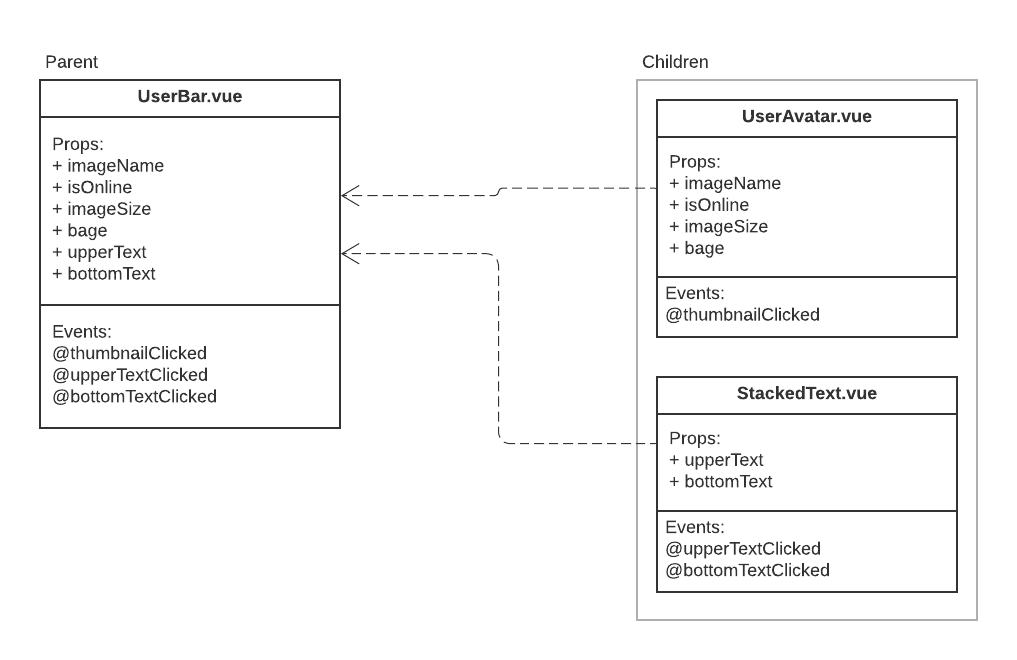
\includegraphics[width=0.75\textwidth]{images/003-000-001-property-hell.png}
	\caption{Abstraktes Beispiel der Property Hell}
	\label{fig:propertyHell}
\end{figure}

Abbildung \ref{fig:propertyHell} zeigt eine Eltern-Komponente die aus zwei weiteren Komponenten besteht. Property-Werte der Eltern-Komponente werden an Kinder-Komponenten weitergegeben. Je mehr Properties die Komponenten besitzen, desto unübersichtlicher wird der Code. Um das Beispiel nachvollziehbar darzustellen, wurden die Property-Namen und Events in allen Komponenten gleich genannt. In den orginallen Komponenten können Property-Namen voneinander abweichen und erschweren die Lesbarkeit und Nachvollziehbarkeit ein Komponente zusätzlich.
 
\section{Komponentenmanagement}
\label{sec:componentManagement}
Bisher wurden Komponenten gemäß dem Atomic Design Prinzip von \cite{AtomicDesign} entwickelt und geordnet. Dabei werden Komponenten in die Kategorien „Atom“, „Molekül“, „Organismus“, „Template“ und „Page“ kategorisiert. Dabei haben sich für dieses Projekt zwei Schwächen herausgestellt:
\begin{enumerate}
 \item Der Unterschied zwischen Molekülen und Organismen ist oft für die Komponenten nicht strikt definierbar.
 \item Es kann passieren, dass größere Komponenten, wie beispielsweise Organismen Moleküle benötigen, die sonst keine andere Komponente benötigt. Diese Moleküle werden jedoch in dem Ordner Moleküle abgespeichert, was zu einer Unübersichtlichkeit der Repositories geführt hat. Der folgende Code soll dies veranschaulichen.
\end{enumerate}

\lstinputlisting[caption={components/organisms/Navigation/Navbar.vue}, label={Komponenten Management - Navbar.vue}]{code/003-000_herausforderungen/KomponentenMangement.vue}

\section{Post-Modularisierung von Komponenten}
\label{sec:postSplitting}
Es kommt immer wieder vor, dass Abschnitte einer Vue-Komponente zur Wiederverwendung eines Abschnitts in eine neue Komponente ausgelagert werden sollen. Neben der Herausforderung zugehörige Methoden und Variablen aus der Logik zu herauszufiltern müssen auch bereits spezifische Stylings in großen genesteten SASS-Abschnitten durchsucht und verschoben werden. Dies ist mühsam und fehleranfällig.

\section{Manuelle Dokumentation der Komponenten}
\label{sec:manualDocumentation}
Eine Dokumentation von Komponenten mit Code Beispielen und Property Auflistungen muss manuell vom Entwickler verantwortet werden. Dies führt dazu, dass Dokumentationen durch menschliche Fehler unvollständig, veraltet oder fehlerhaft sind. Zudem ist die manuelle Dokumentation aufwendig.
 
\section{Abhängigkeit der Portal-Konfiguration in portal-global-components}
\label{sec:portalConfigDep}
Jede Portal Instanz wird im portal-frontend-Repository konfiguriert und dort in einer Datei gespeichert. Das Repository portal-global-components ist zur Verwendung auf eine gültige Portal-Konfiguration aus portal-frontend angewiesen. Dadurch sind die Komponenten in Zukunft nicht in anderen Projekten ohne eine solche Portal-Konfiguration nutzbar.

\chapter{Erstellung der neuen Komponentenbibliothek}
\label{cha:Neue Komponentenbibliothek}

\section{Anforderungen}
Die derzeit eingesetzte Komponentenbibliothek aus dem Repository \textit{portal-global-components} wurde zuerst auf Basis von vue-cli 2 und nach späterer Migration auf vue-cli 3 entwickelt. Es werden bis jetzt keine Dokumentations-Frameworks verwendet und die Dokumentierung der erstellten Bibliothek wird manuell als eigene Vue-App entwickelt.

Aufgrund der bestehenden Komplexität, die unteranderem Resultat der in Kapitel \ref{cha:Herausforderungen im Frontend} aufgelistet Herausforderungen ist, und dem bevorstehenden  UI-Redesigns des gesamten Portals soll eine neue Komponentenbibliothek der Frontend-Infrastruktur hinzugefügt werden. Diese soll zu einer Verbesserung der in Kapitel \ref{cha:Herausforderungen im Frontend} genannten Herausforderungen beitragen und außerdem das Utility-Class Framework Tailwind CSS verwenden und somit im Frontend einführen. Sowohl die bestehende Bibliothek als auch die neue Bibliothek sollen zunächst im Frontend verwendet werden. Ab Release der neuen Bibliothek soll diese jedoch das \textit{portal-global-components} Repository langfristig vollständig ersetzen.

Anforderungen, die sich für die neue Vue-Komponentenbibliothek ergeben sind folglich:
\begin{itemize}
    \item \textbf{Einführung von Tailwind CSS}: Unter Verwendung der Bibliothek wird Tailwind CSS auch in \textit{portal-frontend} eingeführt. Die Bibliothek liefert eine Standard-Tailwind-Konfiguration, die in Portal-Instanzen individuell angepasst werden kann.
    \item \textbf{Isolierte Komponentenentwicklung}: Die Komponenten sollen unabhängig von \textit{portal-frontend} und einer Portal-Koniguration entwickelt werden sowie nutzbar sein (vgl. Abschnitt \ref{sec:portalConfigDep}).
    \item \textbf{Automatisierte Komponentendokumentation}: Die Komponenten sollen nicht mehr vollständig manuell von Entwickelnden dokumentiert werden. Stattdessen soll der Entwickler eine \textit{Single-File-Component} mit mindestens einem Codebeispiel neu einführen können. Anschließend sollen dann beispielsweise Properties und Codebeispiele benutzerfreundlich in einer Vue-Single-Page-Application dargestellt werden \ref{sec:manualDocumentation}).
    \item \textbf{Einfache Komponentenkategorisierung}: Komponenten sollen weiterhin gemäß ihrer Komplexität in entsprechende Ordner gespeichert werden. Die Probleme aus Abschnitt \ref{sec:componentManagement}) sollen dabei weitesgehend gelöst werden.
  \end{itemize}

\section{Frameworkwahl}
Damit die neue Bibliothek möglichst robust ist und die Einführung möglichst einfach umzusetzen ist, soll ein passendes Framework als Projektbasis eingesetzt werden. Zunächst wird ein Vergleich zwischen drei möglichen Frameworks präsentiert um schließlich eine Auswahl treffen zu können.

\subsection{Vergleich}
\label{sec:frameworkComparision}
Nach einer Recherche wurden für dieses Projekt drei Open-Source Frameworks näher betrachtet.

\defcitealias{VueStyleguidist}{\usebibentry{VueStyleguidist}{title}}
\defcitealias{VueDesignSystem}{\usebibentry{VueDesignSystem}{title}}
\defcitealias{Storybook}{\usebibentry{Storybook}{title}}

\begin{enumerate}
    \item \textbf{\citetalias{VueStyleguidist}} (1,8k Follower auf \cite{VueStyleguidistGithub})\newline
    Vue-Styleguidist ist ein Fork des bekannten react-styleguidist (9,2k Follower auf \cite{ReactStyleguidistGithub}). Vue Styleguidist wird offiziell als \emph{``Isolated Vue component development environment with a living style guide.''} \citep{VueStyleguidist} beschrieben. Das Framework kann basierend auf Code-Kommentare einer Komponente eine Dokumentation dieser automatisiert anfertigen. Dokumentationsseiten werden in Markdown verfasst. Außerdem ist dieses Framework offiziell Teil des Vue-Community-Ecosystems\footnote{ \url{https://vue-community.org/guide/ecosystem/documentation.html\#vue-styleguidist } }, was einen langen Support mit regelmäßigen Updates wahrscheinlich macht.
    \item \textbf{\citetalias{VueDesignSystem}} (1,9k Follower auf \cite{VueDesignSystemGithub})\newline
    Das Vue Design System wurde von Viljami Salminen, einem Design System Architekten aus Finland, erstellt und wurde bereits in der Vergangenheit von der AVACO GmbH für eine neue Bibliothek in Betracht gezogen. Das Projekt basiert auf Vue.js und Vue-Stylguidist. Dabei unterscheidet es sich besonders darin eigene Design-System-Praktiken und Strukturen dem Anwendenden anzubieten. Eine Praktik stellt dabei eine abstraktere Atomic Design Alternative dar. Diese ist besonders im Hinblick auf Komponentenmanagement Herausforderung aus Abschnitt \ref{sec:componentManagement} interessant.

    Die Terminologie des abgewandelten Atomic Design Ansatzes werden wir folgt definiert \citep{VueDesignSystemTerminology}:
    \begin{itemize}
        \item \textbf{Design Tokens}: Werden in einer .yml Datei definiert und sind im gesamten Design System als SASS-Variablen nutzbar.
        \item \textbf{Elements}: Komponenten, die nicht weiter heruntergebrochen werden können. Beispielsweise Buttons.
        \item \textbf{Patterns}: Komponenten, die aus anderen \textit{Elements} und \textit{Tokens} bestehen.
        \item \textbf{Templates}: Komponenten, die aus \textit{Elements}, \textit{Patterns} und \textit{Tokens} bestehen
    \end{itemize}

    Der letzte Release erfolgte im Jahr 2018 weshalb man derzeit nicht beurteilen kann inwieweit das Projekt noch gepflegt werden wird. Vue-Styleguidst, das Basisframework, erhält jedoch weiterhin Updates.
    \item \textbf{\citetalias{Storybook}} (53,7k Follower auf \cite{StorybookGithub})\newline
    Storybook ist ein populäres aus der React-Community entstandendes Framework. Die offizielle Beschreibung lautet wie folgt:

    \begin{quotation}
        \emph{``Storybook is an open source tool for developing UI components in isolation for React, Vue, Angular, and more. It makes building stunning UIs organized and efficient.''} \citep{Storybook}
    \end{quotation}

    Obwohl das Framework ursprünglich für React entwickelt wurde unterstützt es mittlerweile in weiten Umfängen viele weitere Frameworks. Komponenten werden dabei in \textit{Stories} dokumentiert, welche in einer eigenen JavaScript-Datei gespeichert werden. Eine Vue-Story wird dann als Stringified Single Page Component verfasst. Dieser Prozess ist nicht vollkommen automatisiert, da zu einer neuen Komponente zunächst eine Story verfasst werden muss. Die Story kann in Form eines Beispielcodes verfasst werden. Jede Komponente, die in eine Story als Modul hineingeladen wird, wird dann automatisiert analysiert und Properties, Slots, etc. benutzerfreundlich dargestellt.

    Insgesamt ist Storybook durch seine Schnittstellen und Pluginsystem sehr mächtig. Dies geschieht jedoch auf Kosten der initialen Aufsetzung.

    Zwei weitere interessante Eigenschaften sind zum einen die Svelte\footnote{ Mehr zu Svelte: \url{https://svelte.dev/} } Unterstützung und zum anderen die Figma-Einbindungsmöglichkeit, da die AVACO GmbH diese beiden Werkzeuge in Zukunft zusätzlich einführen könnte.
\end{enumerate}

\subsection{Auswahl Storybook}
\cite{WorkshopStorefront} definiert in seinem Artikel die Bezeichnungen \textit{Workshop} und \textit{Storefront} in Bezug auf Design-Systeme. Demnach sind \textit{Workshops} Entwicklungsumgebungen für das effektive Erstellen neuer UI-Komponenten im Team. Der \textit{Workshop} bietet alle Werkzeuge und Strukturen für diese Arbeit.

Die \textit{Storefront} präsentiert hingegen das fertige Design-System mit allen weiteren Ressourcen. Ähnlich zu einem Styleguide sollen in der \textit{Storefront} Informationen erscheinen, die für Entwickler und Benutzer aus anderen Disziplinen hilfreich sind.

Laut \cite{StorybookVSStyleguidist} dem Initiator von Storybook haben Styleguidist und Storybook viele Gemeinsamkeiten und bedienen beide jeweils Anforderungen an Workshop und Storefront. Jedoch klassifiziert er letztendlich Styleguidist als Storefront und Storybook als Workshop. Auch \cite{FrostCite} bezeichnet Storbook wie folgt:
\begin{quotation}
    \emph{``Storybook is a powerful frontend workshop environment tool that allows teams to design, build, and organize UI components (and even full screens!) without getting tripped up over business logic and plumbing.''}
\end{quotation}
Da es in diesem Projekt besonders darum geht eine robuste Komponentenbibliothek für Frontend-Entwickler zu erstellen, welche die Entwickler in ihren Entwicklungen unterstützt und die Entwickler nur einfache Storefront-Eigenschaften benötigen wird das Projekt mit Storybook entwickelt. Jedoch sollen die von \citep{VueDesignSystemTerminology} definierten Terminologien und Prinzipien bei der Umsetzung auf das Tailwind-Ecosystem projiziert werden. Sofern in Zukunft die Bibliothek um ein vollständiges Design System erweitert werden sollte, sollte ein zusätzliches Werkzeug zur Dokumentierung und Darstellung des Systems gesucht werden.

\section{Entwicklung}
\subsection{Repositoryverwendung}
Die Komponenten Bibliothek wird in einem eigenen Repository unter dem Namen \textit{portal-storybook} erstellt und kann anschließend als \textit{Node-Module} in anderen Projekten als Vue-Plugin installiert werden. Dabei soll die Bibliothek drei unterschiedliche Komponenten-Registrierungen ermöglichen.

\begin{enumerate}
    \item \textbf{Installation aller Komponenten im globalen Vue Namespace}: Komponenten müssen zur Verwendung nicht mehr in andere Dokumente importiert werden, sondern können direkt im Markup unter ihrem Komponenten-Namen genutzt werden.
\begin{lstlisting}[language=JavaScript , caption={Globale Installierung},label={lst:GlobalInstall}]
// bspw. main.js in einem vue-cli-3 Projekt
// ...
import * as storybook from 'portal-storybook'
// ...
Vue.use(storybook, {useAllComponents: true})
\end{lstlisting}
    \item \textbf{Installation einzelner Komponenten als Modul durch \textit{Named Exports} aus der Dependency heraus}: Komponenten werden nicht im globalen Namespace installiert sondern werden erst spezifisch in den Dokumenten wo sie genutzt werden durch \textit{Named Imports} als Komponente installiert. In der \textit{main.js} aus \ref{lst:GlobalInstall} würde jedoch weiterhin \textit{Vue.use(storybook, {})} ohne dem useAllComponents-Key aufgerufen werden um andere notwendige Abhängigkeiten zu registrieren. 
\begin{lstlisting}[language=JavaScript , caption={Named Exports/Imports in einer SFC},label={lst:NamedExports}]
// bspw. eine Datei mit dem Namen Dashboard.vue im
// ...
<script>
import { MyComponent1, MyComponent2 } from 'portal-storybook'

export default {
    components: { MyComponent1, MyComponent2 } 
}
</script>
\end{lstlisting}
    \item \textbf{Installation einzelner Komponenten als Modul durch import der SFC Vue-Dateien aus dem Dependecy-Verzeichnis}: Sofern Treeshaking in einem Projekt nicht unterstützt wird und eine globale Installation nicht erfolgen soll können Komponenten außerdem auch durch einzelne Imports installiert werden.
\begin{lstlisting}[language=JavaScript , caption={Default Exports/Imports in einer SFC},label={lst:NamedExports}]
// bspw. eine Datei mit dem Namen Dashboard.vue im
// ...
<script>
import MyComponent1 from 'portal-storybook/src/elements/MyComponent1'
import MyComponent1 from 'portal-storybook/src/elements/MyComponent2'

export default {
    components: { MyComponent1, MyComponent2 } 
}
</script>
\end{lstlisting}
\end{enumerate}
\subsection{Repositoryaufbau}
Wie bereits im Vorwort erwähnt wird in dieser Arbeit nicht das Orginal-Repository \textit{portal-storybook} aus dem Firmeneigentum der AVACO GmbH referenziert sondern eine andere Komponentenbiliothek (\textit{tailwindstories}) die auf den selben Konzepten und Lösungen aufbaut, nicht die Firmenkomponenten enthält und neu aufgetauchte Probleme aus \textit{portal-storybook} (vgl. \ref{sec:newChallenges}) bereits mitbehandelt.

Die Abbildung \ref{fig:repoStorybook} am Ende dieses Kapitels zeigt einen Screenshot des \textit{tailwindstories}-Repository und stellt den Verzeichnisaufbau nach der Einführung von storybook in ein neues \textit{vue-cli-3} Vue-Projekt (v.2.) da.

Neben diversen Konfigurationsdateien gibt es die folgenden hervorzuhebenden Verzeichnisse und Dateien:
\begin{itemize}
    \item \textbf{.storybook}\newline
    Enthält alle Storybook spezifisch Workbench-Konfigurationen und Funktionen. Diese sind wichtig für die Nutzung der Workbench, werden aber für den Import fertiger Komponente in einem anderen Projekt nicht benötigt.
    \item \textbf{src/main.js}\newline
    Entrypoint-Datei für die Nutzung als Bibliothek mit Setup-Methoden und Bibliothek-Konfigurationen.
    \item \textbf{src/elements}\newline
    Verzeichnis mit Komponenten die als \textit{elements} klassifiziert werden. Komponenten werden als Vue-SFC-Dateien angelegt, in der index.js importiert und dann als Named-Modul in der main.js importiert. Eine README.md erklärt die Klassifizierungsmerkmale laut Salminen:
    \begin{quotation}
        \emph{``Elements utilize decisions made on the token level. A simple example of an element would be a button, a link, or an input. Anything that cannot be broken down further. I use the name ‘element’ since everything in Vue and React world is nowadays ‘a component.’ Using that term for anything else would be confusing.''} \citep{VUEDSElements}
    \end{quotation}
    \item \textbf{src/patterns}\newline
    Verzeichnis mit Komponenten die als \textit{patterns} klassifiziert werden. (wie \textit{src/elements})
    \begin{quotation}
        \emph{``Patterns are UI Patterns that fall on the more complex side of the spectrum. So for example things like a date picker, a data table, or a visualization. Patterns utilize both elements and tokens. 
        If you wonder whether something should be called an element or a pattern, ask yourself this question: “Can this be broken down into smaller pieces?” If the answer is yes, it should most likely be a pattern.''} \citep{VUEDSPatterns}
    \end{quotation}
    \item \textbf{src/templates}\newline
    Verzeichnis mit Komponenten die als \textit{templates} klassifiziert werden. (wie \textit{src/elements})
    \begin{quotation}
        \emph{``Templates exist to document the layout and structure of a section. I am not calling these pages since semantically that would be incorrect. While they can be pages, that’s not their only functionality. Templates consist of the three things mentioned above: tokens, elements, and patterns.''} \citep{VUEDSTemplates}
    \end{quotation}
    \item \textbf{src/plugins}\newline
    Verzeichnis mit Tailwind-Plugins die unter anderem als \textit{Tokens} klassifiziert werden können.
    \begin{quotation}
        \emph{``Design tokens are the visual design atoms of the design system — specifically, they are named entities that store visual design attributes. We use them in place of hard-coded values (such as hex values for color or pixel values for spacing) in order to maintain a scalable and consistent visual system for UI development.''} \citep{DesignTokens}
    \end{quotation}
    Die Tailwind CSS Plugins können Tokens als neue Utility-Klassen einführen.\footnote{Mehr zu Tailwind CSS Plugins: \url{https://tailwindcss.com/docs/plugins}}
\end{itemize}

\begin{figure}[!ht]
	\centering
		%[natürliche Breite in Pixeln, natürliche Höhe in Pixeln, Abhängigkeit von der Textbreite]
		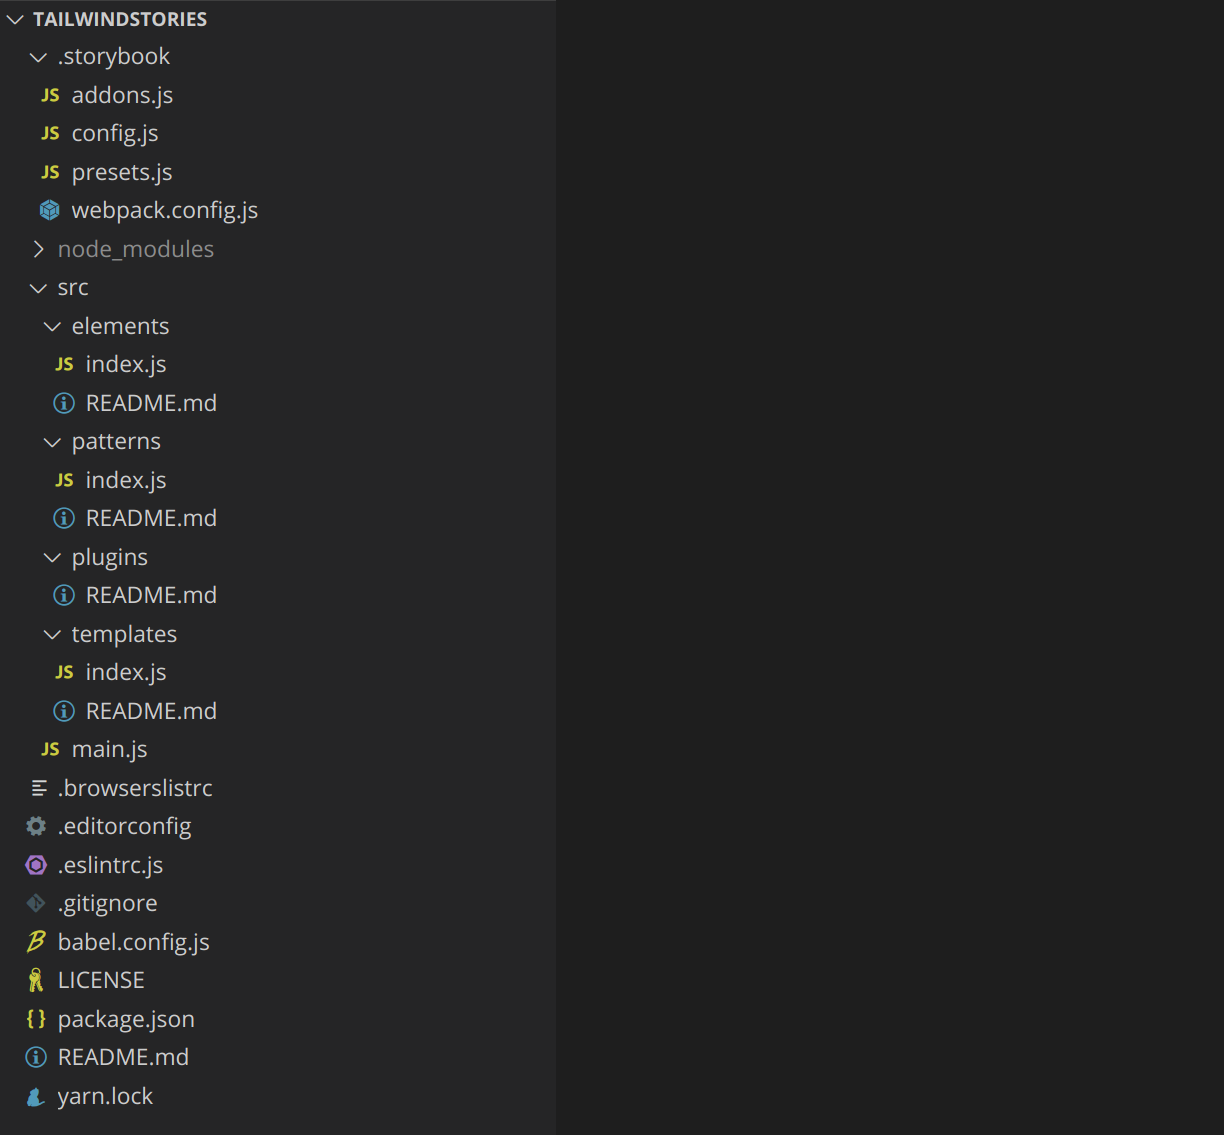
\includegraphics[width=.85\textwidth]{images/004-000-001-repo-storybook.png}
	\caption{Repositoryaufbau mit Storybook}
	\label{fig:repoStorybook}
\end{figure}

\subsection{Storybook Setup}
\label{sec:storybooksetup}
Zu Beginn des Projektes wurde Storybook Version 4 in \textit{portal-storybook} installiert und eingesetzt. Zur automatisierten Dokumentation der erstellten Vue-Komponenten wurde das Addon \textit{storybook-addon-vue-info}\footnote{Repository: \url{https://github.com/pocka/storybook-addon-vue-info}} eingesetzt. Dieses Addon kann die genutzten Komponenten in einer Story analysieren und wichtige Eigenschaften sowie den Quellcode in dem Storybook-GUI nutzerfreundlich darstellen.

Seit der Storybook Version 6 wird das Storybook Addon \textit{@storybook/addon-info} auf welchem das Addon \textit{storybook-addon-vue-info} basiert nicht mehr unterstützt und Storybook bietet nun offiziell das Addon \textit{@storybook/addon-docs} für den Zweck automatisierter Komponenten-Analysen an. Dieses Addon arbeitet derzeit besonders gut mit React Komponenten aber auch Vue Komponenten können analysiert und mit ihren Eigenschaften dargestellt werden. Es gibt die Möglichkeit Property-Werte direkt aus der GUI heraus zu manipulieren. Der einzige Nachteil im Vergleich zu dem nun veralteten (deprecated) \textit{storybook-addon-vue-info} ist, dass Code-Snippets derzeit nicht den eigentlichen Code der dargestellten Komponente enthalten, sondern den Code der Story \citep{GithubIssueStorybook}. In React mit JSX tritt dieses Problem jedoch nicht auf.

Da dies jedoch für eine gute Developer-Expierence behindernd ist, wurde \textit{tailwindstories} zunächst auch nicht auf der Storybook Version 6 aufgebaut sondern auf der Version 5 zusammen mit \textit{storybook-addon-vue-info}. In der Zukunft soll jedoch ein Upgrade auf Version 6 mit \textit{@storybook/addon-docs} ausgeführt werden.


\chapter{Einführung von Tailwind CSS}
\label{cha:Tailwindcss}
Tailwind CSS ist ein CSS Framework, dass auf eine \textit{Utlity-First} Methodik basiert. Dabei werden CSS-Klassen überwiegend als atomare Attribute definiert, die anschließend bei Bedarf in Komponenten-Klassen abstrahiert werden können.

\section{Allgemeine Vorteile}
\begin{quotation}
	\emph{``We’ve had great success with going utility-first in the Algolia documentation, reducing our CSS from over 125 KB (and continuously growing) to less than 50 KB (9 KB GZipped, 7 KB with Brotli compression), \textbf{which represents a 60\% size decrease!} From a user perspective, this is a guarantee of lightning-fast loading styles with extremely low overhead.''}
	\citep{AlgoliaTailwindBlog}
\end{quotation}
Die Vorteile von Tailwind CSS gegenüber anderer CSS-Frameworks sind vielseitig. Einige der von \cite{AlgoliaTailwindBlog} hervorgehobenen Eigenschaften sind insbesondere:
\begin{itemize}
  \item \textbf{Anpassbarkeit und Nachvollziehbarkeit}: Utility Klassen werden in einer JavaScript-Datei definiert und sind somit zentral einsehbar, was einfacher und schneller zu warten ist und eine gute Anpassbarkeit an individuelle Design-Systeme ermöglicht. Die Dokumentation von Tailwind CSS ist außerdem leicht verständlich für Lernende.
  \item \textbf{Kontrollierbare Dateigröße}: Durch einmalig definierte Utility Klassen wächst der CSS Code nicht mehr an. Styles müsssen nicht mehr durch Spezifitäten überschrieben werden, was bessere Performance bewirkt.
  \item \textbf{Automatisierte \textit{CSS-Spülung}} (engl. purge): Da Tailwind CSS initial viele zunächst ungenutzte Utility-Klassen basierend aus einer Konfiguration erstellt (Initial Größe beträgt meist unkomprimiert c.a. 3400 kB\footnote{vgl. \url{https://tailwindcss.com/docs/controlling-file-size}}) wurde das Framework mit dem Framework PurgeCSS für die Generierung von Production-Code erstellt. PurgeCSS vergleicht die gesamte Codebasis mit allen CSS-Klassen und entfernt CSS-Klassen die nicht genutzt wurden. Dadurch wird die CSS-Dateigröße meistens auf c.a. 10kB (komprimiert) reduziert \citep{TailwindcssDocsFileControll}.
  \item \textbf{Komprimierungsfreundlichkeit}: Durch Tailwind CSS erfolgt die eigentliche Produktgestaltung meist direkt im Markup Code unter redundanter Verwendung von Utility-Klassennamen. Komprimierungsalgorithmen sind so gestaltet das gleiche Strings komprimiert werden, wodurch der Markup-Code durch Utlity-Klassen unwesentlich größer wird.
\end{itemize}

\section{Chanceneinschätzung für My.PORTAL}
\label{sec:Chanceneinschtzung}
Durch die Einführung von Tailwind CSS erwartet die AVACO GmbH die folgenden Probleme (vgl. Kapitel \ref{cha:Herausforderungen im Frontend}) zu lösen oder zu verbessern:

\begin{itemize}
  \item \textbf{Redundante CSS Definitionen}: Scoped-CSS wird durch Tailwind CSS auf ein Minimum reduziert. Redudante CSS Defintionen sollten (nahezu) vollständig entfernt werden können.
  \item \textbf{Ungenutzte CSS Klassen}: Neben Tailwinds Utlity-Klassen wird es nur in Ausnahmen andere Klassen geben. Die Chance, dass ungenutze CSS Klassen geschrieben werden wird deutlich reduziert. Ungenutze Tailwind-Klassen werden automatisch von PurgeCSS entfernt.
  \item \textbf{Post-Modularisierung von Komponenten}: Da die Styledefinitionen sich im Markup als CSS Klassen befinden sollte ein Verschieben von Code Abschnitten nur noch eine Analyse des Markups und der Script-Logik erfordern.
  \item \textbf{Tailwindkonfiguration statt Portalkonfiguration in portal-storybook} (vgl Abschnitt \ref{sec:portalConfigDep}): Es wird keine Portal-Konfiguration für die Bibliothek benötigt. Stattdessen enthält die Bibliothek eine eigene \textit{tailwind.conf.js} die sich nach der Tailwind CSS Dokumentation ausrichtet. Andere Projekte nehmen diese Konfiguration dann als Basis und können sie entsprechend eigener Anforderungen zielgerichtet anpassen. (vgl. \ref{sec:ProjectCustomisation})
  \item \textbf{Property Hell}: Tailwind CSS löst Vue-Properties ab die bisher dynamisch Klassen mit höherer Spezifität zur umgestaltung einer Komponentenerscheinung angelegt wurden. Stattdessen sollen Erscheinungsanpassungen mit Utility-Klassen in \textit{class}-Attributen erfolgen. Die Property Hell wird in Kapitel \ref{sec:propertyHellSolution} näher betrachtet.
\end{itemize}

Diese Einführung ist jedoch auch mit Risiken verbunden:
\begin{itemize}
  \item \textbf{Wenig allg. Langzeiterfahrung mit Tailwind CSS}: Unbekannte Probleme können in der Tailwind-Community oder spezifisch bei der AVACO GmbH auftreten. Jedoch fällt in der Entwickler-Community  aktuell Tailwind CSS verglichen mit anderen populären Frameworks (bspw. Bootstrap) auf den höchsten Zufriedenheitsgrad \citep{StateCSS2019_Frameworks}.
  \item \textbf{Technologie Konflikte}: Besonders in der Übergangsphase werden alte Technologien (z.B. SASS und Bootstrap) zusammen mit Tailwind CSS und PostCSS (inkl. PurgeCSS) im Projektcode koexistieren. Die Folgen dessen können sich im Hinblick auf Bugs, Performance und Code-Komplexität stärker oder schwächer auswirken.
  \item \textbf{Bevorstehendes Upgrade auf Node 12}: Derzeit wird das Frontend auf der Node Version 11 aufgesetzt. Mit dem nächsten großen Release wird Tailwind CSS Version 2 nur noch Node ab den Versionen 12 unterstützen. Da jedoch die Gebundenheit von My.PORTAL zu Version 11 derzeit primär von SASS abhängt und SASS langfristig durch Tailwind CSS und PostCSS ersetzt werden wird, ist dies kein dauerhafter Risikozustand.
\end{itemize}

\section{Entwicklung}
Das Setup erfolgte gemäß der offiziellen Dokumentation\footnote{vgl. \url{https://tailwindcss.com/docs/installation}} von Tailwind CSS. Damit diese Komponenten sich in anderen Projekten richtig verhalten, muss Tailwind CSS auf Basis der tailwind.config.js in diesen verfügbar sein und die tailwind.css Datei aus der Bibliothek importiert werden. (vgl. Abschnitt \ref{sec:ProjectCustomisation})


\subsection{Plugins}
Die Tailwind Standardkonfiguration soll durch Plugins und Wertüberschreibung an Design-Systeme anpassbar sein. Aktuell gibt es drei Plugins:

\begin{itemize}
  \item \textbf{Color-Plugin}: Führt Corporate Identiy Farben als Utlity-Klassen ein. Es kann eine Primary Color gesetzt werden aus welcher automatisch eine passende Farbpalette für Status-Farben (Success, Error, ...) erzeugt wird. Als Basis wurde das Paket \textit{chroma-js} gewählt welches die Farbpaletten im LAB-Farbraum mischt\footnote{chroma-js LAB: \url{https://gka.github.io/chroma.js/\#chroma-lab}}. Da dieses Plugin die Konfiguration mit weiteren Object-Keys erweitert, wird es in der Konfigurationsdatei nicht als Plugin registriert sondern wird dem Konfigurationsobjekt per Spread-Syntax angehangen.
  \item \textbf{Container-Plugin}: Führt responsive Margin/Padding Größen für Container ein. Die Utility-Klasse \textit{.px-c} setzt das Padding eines Layout-Containers. Dies bietet eine größere Flexibilität beim entwickeln von Markup unter Einhaltung von Linienführungen in dem GUI.
  \item \textbf{Box-Plugin}: Definiert das Aussehen von GUI-Boxen (z.B. Karten) indem es Box-Utilitly-Klassen und eine Komponenten-Klasse (\textit{.box}) einführt.
\end{itemize}

\subsection{Anpassungsmethode in Projekten}
\label{sec:ProjectCustomisation}

Damit die Komponenten sich in die diversen Erscheinungen unterschiedlicher Portal Instanzen einpassen können, wurde eine Tailwind Setup-Methode angefertigt. Diese gibt das der Komponentenbibiliothek zugrundeliegende Tailwind-Konfigurationsobjekt zurück und bietet durch definierte Parameter die Möglichkeit das Erscheinungsbild (derzeit die Farbpalette) zu verändern. Eine tiefere Anpassung ist durch normale Tailwind Konfiguration möglich, indem Werte der Bibliothekskonfiguration verändert, entfernt oder erweitert werden. Die folgenden Codebeispiele referenzieren das Repository \textit{tailwindstories} (vgl. Vorbemerkung der Arbeit).

\lstinputlisting[caption={tailwind.config.js in einem Vue-Cli 3 Projekt}, label={tailwind.config.js}]{code/005-000_tailwindcss/tailwind.config.js}

\lstinputlisting[caption={Erweiterte tailwind.config.js in einem Vue-Cli 3 Projekt}, label={tailwind.config.js}]{code/005-000_tailwindcss/tailwind.advanced.config.js}

\subsection{My.Portal Konfiguration}
In einem einfachen Vue-Cli 3 Projekt ist das Setup von Postcss und Tailwind allgemein gut dokumentiert verfügbar\footnote{vgl. \url{https://cli.vuejs.org/guide/css.html\#postcss} und \url{https://tailwindcss.com/docs/installation}}. Die MyPortal Vue-Applikation basiert jedoch noch auf vue cli 2 mit diversen individuellen Webpack Konfigurationen sowie Transpilierungsskripten die auf dem Vue Webpack Template aufbauen\footnote{vgl \url{http://vuejs-templates.github.io/webpack/}}. Wie bereits in Abschnitt \ref{sec:portalConfigDep} erwähnt enthält das Hauptrepository zudem die einzelnen Instanzkonfigurationen.

Die Struktur ist in Abbildung \ref{fig:structureDir} modelliert. In Englisch beschriebene Abschnitte stammen von der Webpack-Template Dokumentation und der \textit{portals} Ordner enthält die Instanzspezifischen Konfigurationen. Der Struktur wurde außerdem bereits eine \textit{tailwind.config.js} angehängt auf welche im Folgenenden eingegangen wird.

\begin{figure}[!ht]
	\centering
		%[natürliche Breite in Pixeln, natürliche Höhe in Pixeln, Abhängigkeit von der Textbreite]
		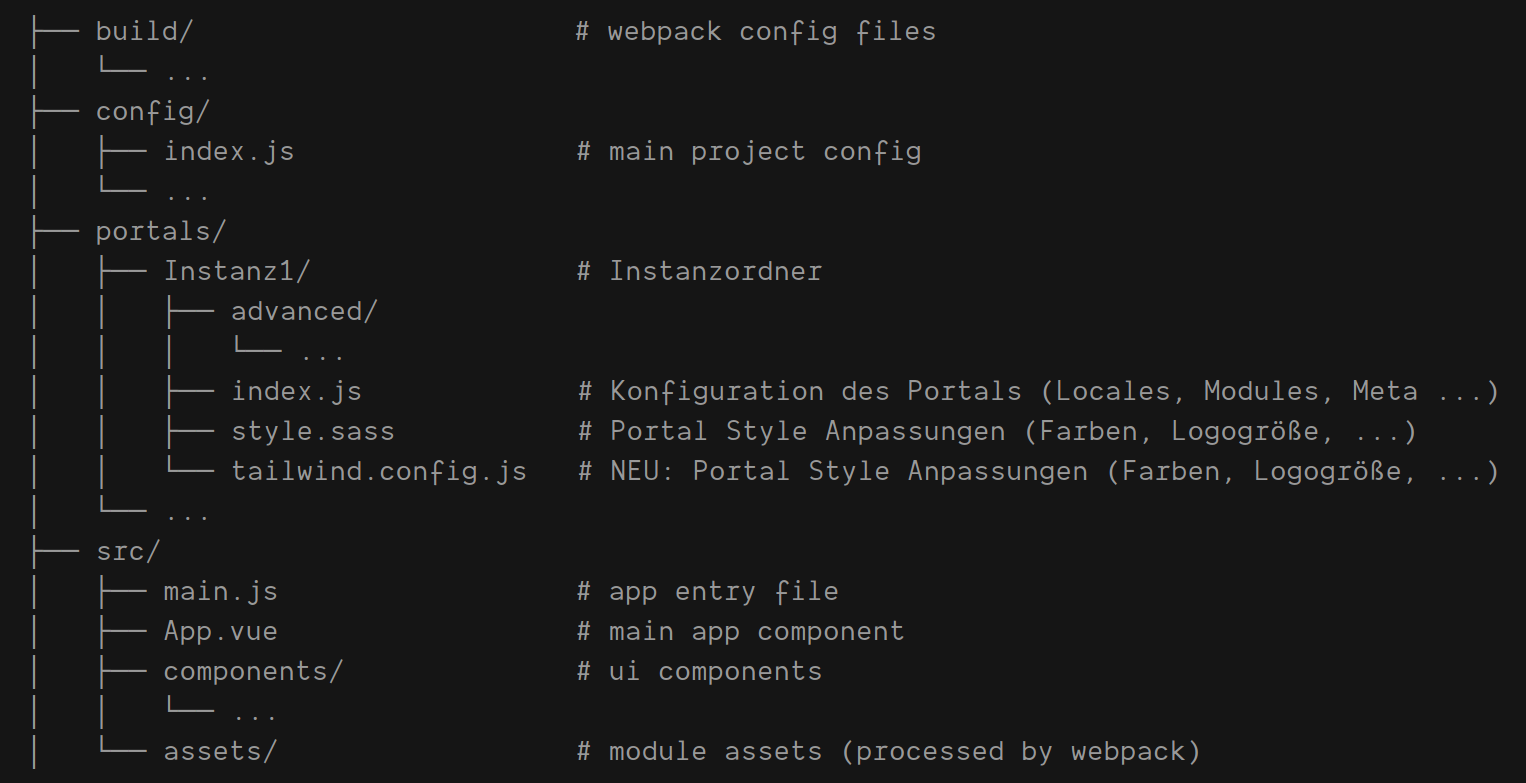
\includegraphics[width=.85\textwidth]{images/005-000-001-structureDir.png}
	\caption{Portal-Frontend Repository Struktur}
	\label{fig:structureDir}
\end{figure}

Ein Portal kann anschließend durch ein Node-Skript mit einem Portalordnernamen als Parameter transpiliert werden:

\begin{quotation}
	\emph{npm run build Instanz1}
\end{quotation}

Durch den Befehl werden die Dateien aus dem Ordner \textit{Instanz1} in die Build und Konfigurationsdateien importiert. Äquivalent könnte man eine neue Portalinstanz in dem Verzeichnis \textit{portals/Instanz2} anlegen und starten.

Da Tailwind CSS standardmäßig im Root Verzeichnis nach der optionalen \textit{tailwind.config.js} sucht sind für diese Art der Instanziierung besondere Anpassungen für das Tailwind Setup im \textit{portal-frontend} notwendig.

Dazu wurde zunächst im \textit{build} Verzeichnis ein Modul anlegt, die eine normale Tailwindkonfiguration anhand des Portalnamens auflösen kann und mit der Tailwindkonfiguration aus der Komponentenbibliothek zusammenführt sowie ein erweitertes PurgeCSS Setup festlegt (vgl. Codebeispiel \ref{tailwind.js}).

\lstinputlisting[caption={Modul zur Auflösung und Zusammenführung der tailwind.config.js}, label={tailwind.js}]{code/005-000_tailwindcss/tailwind.js}

Damit dieses Modul nun für das Setup von Tailwind CSS innerhalb von PostCSS angewandt wird muss die \textit{postcss.config.js} wie folgt angepasst werden.

\lstinputlisting[caption={Modul zur Auflösung und Zusammenführung der tailwind.config.js}, label={tailwind.js}]{code/005-000_tailwindcss/PostcssConf.js}

Dabei ist das Setup in Form eines Rückgabewertes einer Funktion für PostCSS nicht so häufig verbreitet. Grund dafür ist jedoch das benötigte \textit{Context (ctx)} Objekt\footnote{vgl. \url{https://github.com/postcss/postcss-load-config\#context}} was in der Webpack Konfiguration wie folgt definiert wurde:

\lstinputlisting[caption={Webpack.conf.js}, label={webpack.conf.js}]{code/005-000_tailwindcss/Webpack.conf.js}
\chapter{Resultate}
\label{cha:Ergebnisse}

\section{Chancenbewertung Tailwind CSS}
Der folgende Abschnitt bewertet die in Abschnitt \ref{sec:Chanceneinschtzung} gelisteten Chancen und Risiken im Hinblick auf die derzeitige Implementierung von Tailwind CSS.
\subsection{Redundante CSS Definitionen}
\label{subsec:redundantCSS}
Durch den Einsatz von Tailwind CSS wird ein Alternative gegenüber der Nutzung von SASS-Mixins geschaffen. Da SASS nach dem Tailwind CSS Refactoring vollständig entfernt werden wird sind Entwickler bereits jetzt dazu angehalten keine Mixins mehr zu verwenden.

Um Einschätzen zu können inwieweit sich das Entfernen von Mixins lohnt wurde eine exemplarische Berechnung des von \textit{+make-col()} erzeugten Codes angefertigt.

Mit dem Wissen, dass die drei Displaygrößen Mobile, Tablet und Desktop im Projekt unterschiedliche Spezifitäten haben müssen führt der Einsatz des Mixins zu redundanten Code, der sich derzeit mit äquivalenten Utility-First CSS Klassen um c.a. 88 - 90\% reduzieren ließe. 

\begin{quotation}
	\textbf{10 Parameterwerte * 3 Screengrößen = 30 Klassen bzw. bei 12 Parameterwerten wären es dauerhaft 36 Klassen} (vgl. \ref{sec:redundantCSS})
\end{quotation}

Somit versursacht der Einsatz dieses Mixins allein 34 KB (28KB minified) (bezogen auf 303-maligen Gebrauch). Das Tailwind CSS Äquivalent hat jedoch lediglich eine Größe von 3,9 KB (3,3KB minified).

Da bisher noch kein vollständiges Refactoring des Frontends umgesetzt wurde, sondern diese Arbeit sich mit der Umsetzung einer geeigneten Komponentenbibliothek sowie der generellen Einführung von Tailwind CSS befasst, kann die gesamte CSS-Ersparnis im Vergleich zu SASS noch nicht ermittelt werden. Jedoch ist das Portal-Frontend durchaus komplexer als die ehemalige Algolia-Dokumentation \citep{AlgoliaTailwindBlog} gestaltet, weshalb man ziemlich sicher von einer ähnlich guten Einsparung von 60\% Code ausgehen kann.

\subsection{Ungenutzte CSS Klassen}
\label{subsec:unusedCSS}
Diese Chance hat sich durch Tailwind CSS und PurgeCSS bewahrheitet. Ungenutzte CSS Klassen werden durch \textit{PurgeCSS} entfernt. Jedoch ist dies nicht die robusteste Art ungenutzten Code zu behandeln, da der Code immernoch in den Quelldateien verweilt. Durch den vollständigen Wechsel zu Tailwind CSS wird dieser Problematik jedoch ebenfalls entgegengewirkt, da in der Regel keine neuen CSS Klassen definiert werden. Wird ein Markupabschnitt bearbeitet oder entfernt, werden die gesetzten Utility-Klassen gleichmaßen behandelt (entfernt/bearbeitet). Diese Chance hat sich bereits jetzt schon in einigen Komponenten bewahrheitet.

\subsection{Property Hell}
\label{sec:propertyHellSolution}
Der Verhalt bzgl. der Property-Hell hat sich nur teilweise durch Tailwind CSS verbessert. Die Gründe für die Entstehung einer Property Hell sind vielseitig und zunächst nicht durch Storybook oder
Tailwind CSS zu beseitigen. Um eine Verbesserung zu erlangen muss ein anderer Architekturstil von Vue-Komponenten aufgesetzt werden, der einer Property-Orientierung entgegenwirkt.

Eine Alternative zu Properties bieten \textit{Slots}. Anders als Properties werden bei Slots nicht JavaScript-Typen weitergegeben sondern Codeabschnitte definierte in welche weiterer Code eingefügt werden kann \citep{VueDocsSlots}. Durch diese Art der Verschachtelung in der Eltern-Komponente wird ein hindurchreichen von Properties entgegengewirkt. Zudem lässt sich der Inhalt der Slots dynamisch gestalten, was Komponenten deutlich flexibler einsetzen lässt.

\cite{SlotsPropsArticle} befürwortet in seinem Artikel eine ähnliche Herangehensweise. Die Vorteile listet er wie folgt:

\begin{itemize}
  \item \textbf{Flexibilität}: Für neue Slot-Inhalte müssen keine neuen Properties definiert werden.
  \item \textbf{Komponentenweitergabe}: Auch Komponenten können in einen Slot eingefügt werden.
  \item \textbf{Keine If-Statements}: Properties müssen nicht mehr validiert werden.
  \item \textbf{Bessere Lesbarkeit}
\end{itemize}

\lstinputlisting[caption={ChatWindowContacts.vue}, label={ChatWindowContacts}]{code/007-000_ergebnisse/ChatWindowContacts.vue}

Im Codebeispiel wurde außerdem eine \textit{rounedClass} Property eingeführt. Diese dient dazu dynamisch Utility-Klassen an ein Markup-Element zu setzen. Dadurch müssen nicht mehr weiter dynamische Klassen definiert werden wie zum Beispiel eine Klasse \textit{entity--rounded-bigger} die durch eine boolische Property \textit{isRoundedBigger = true} gesetzt werden. Stattdessen kann der Entwickler eine \textit{roundedClass} wie ein normales Class Attribut behandeln, dass \textit{entity} gesetzt wird und den Standardwert mit genau den Werten überschreiben, die in seinem Kontext benötigt werden.

Ein Beispiel wäre, der \textit{Entity} nur die \textit{rounded} Erscheinung auf mobilen Geräten verleihen zu wollen: 

\begin{quotation}
	\textit{roundedClass = "rounded md:rounded-none"} (mit diesem Vorgehen muss der Entwickler keine neue Prop wie \textit{isRoundedOnlyMobile} definieren)
\end{quotation}

\subsection{Post-Modularisierung von Komponenten}
\label{subsec:postSplitting}
Das Verschieben von Markup-Abschnitten zusammen mit Utility-Klassen ist bei weiten nicht mehr so komplex. Jedoch ist es weiterhin schwierig die richtigen Script-Abschnitt herauszufiltern um eine Komponente inkl. Funktionalität zu extrahieren. In Abschnitt \ref{cha:vue3} soll geprüft werden ob Vue Version 3 neue Möglichkeiten bietet, die sich positiv auf diesen Prozess auswirken.

\subsection{Tailwindkonfiguration  statt  Portalkonfiguration  in  portal-storybook}
\label{subsec:tailwindConfVSPortalConf}
Tailwind CSS hat diese Chance letztendlich erfüllt. Die Repositorystruktur ist nun nicht mehr vom Client (portal-frontend) abhängig. Das Setup von \textit{portal-storybook} ist jedoch für ein Projekt wie \textit{portal-frontend} durch die verschiedenen Konfigurationsdateien etwas komplizierter gestaltet als zunächst für Standard-Vue-Applikationen angenommen.

\section{Risikobewertung Tailwind CSS}
\subsection{Technologie Konflikte}
Dieses Risiko hat sich mit der Einführung von Tailwind CSS bewahrheitet. Da die Frameworks Bootstrap und Tailwind CSS beide auf eigenen Reset.css Dateien basieren, die beide die Standardbrowser Styles anpassen, gab es viele Konflikte bei Style-Elementen, wie Überschriften, Textabschnitte, Links und Listen. Da jedoch Tailwind CSS langfristig als Stylebasis dienen soll, war es für My.PORTAL besser die Bootstrap Reset-Styles zu entfernen und die neuen Bugs im Portal manuell mit Tailwind CSS Utility Klassen wieder in die ursprüngliche Erscheinung zu gestalten. Zudem mussten einige Third-Party-Plugins auf CSS-Klassen geprüft werden, die nicht von PurgeCSS entfernt werden dürfen. Dies war zeitaufwendig jedoch auch nicht schwierig.

\subsection{Weitere Risiken}
Inwieweit die geringe Langzeiterfahrung mit Tailwind CSS und das bevorstehende Upgrade auf Node 12 Herausforderungen mit sich bringen, lässt sich schwierig prognostizieren und bewerten. Jedoch soll in Zukunft ein größeres Technologieupgrade im gesamten Portal geschehen, weshalb das Upgrade auf Node 12 ohnehin mittlerweile als Vorteil zu bewerten ist und die Upgrades an sich unter anderem für dieses Projekt als neue Chancen wie Risiken kategorisiert werden können.

\section{Weitere Beobachtung}
Nach der Implementierung und Nutzung von \textit{portal-storybook} konnten unteranderem neue Herausforderungen, Chancen und Risiken aufgedeckt werden.
\subsection{Neue Herausforderungen}
\label{sec:newChallenges}
\begin{itemize}
  \item \textbf{Debugging: Codemarkup identifizieren}: Wenn man transpilierten Code im Browser zum untersuchen identifizieren möchte, kann durch die fehlenden individuellen Klassennamen eine schnelle Identifizierung des gesuchten Codeabschnitts schwierig sein. Ein Hilfe gegen dieses Problem sind der konsequente Einsatz von semantisch richtigen HTML5-Tags, jedoch tritt das Problem dennoch gelegentlich auf.
  \item \textbf{Längere \emph{Build Time} auf Production}: Durch den zusätzlichen Einsatz von PurgeCSS hat sich die Buildtime eines production-stage Portals verdreifacht. Da SASS ebenfalls noch im Portal enthalten ist, ist eine Verbesserung abzusehen, da mit dem entfernen von SASS der Preprozessor und viele CSS Klassen entfernt werden. Jedoch ist es nicht einschätzbar wie positiv der Effekt im Hinblick auf die Build-Time ausfallen wird.
\end{itemize}

\subsection{Neue Chancen und Risiken}
Für Storybook, Tailwind CSS, Node.js und Vue.js stehen Upgrades auf neue Hauptversionen an. Diese Upgrades bringen allgemein neue Features und bessere Performance sind aber auch für eine dauerhafte Aktualität des Portals notwendig. 

\textbf{Tailwind CSS} wird in Version 2 einige Deprecation-Änderungen enthalten, jedoch wird auf diese Änderungen bereits in den aktuellen Versionen hingewiesen und es gibt die Möglichkeit Tailwind bereits mit den neuen Änderungen zu verwenden. 

\textbf{Storybook} wäre bereits möglich zu aktualisieren, allerdings besteht derzeit noch immer das Dokumentationsproblem aus Abschnitt \ref{sec:storybooksetup}. Solange dieses Problem nicht gelöst ist, wäre ein Upgrade unpraktisch. Daher ist dieses Upgrade trotz Chancen auf ein besseres (offizielles) Dokumentationsbild auch als ein Risiko zu betrachten, welches das Aktualisieren generell blockt.

\textbf{Vue.js} Version 3 ist bereits veröffentlicht. Jedoch sind die meisten eingesetzten Vue-Community-Projekte noch nicht entsprechend aktualisiert worden. Die AVACO GmbH plant mit dem Launch von Nuxt.js Version 3, welches auf Vue 3 aufbauen soll, ein Upgrade auf Vue Version 3 mit Nuxt.js zu tätigen.
Mit diesem Upgrade sind viele Chancen und Risiken verbunden, die nicht direkt im Zusammenhang mit Tailwind CSS oder Storybook stehen werden. In Kapitel \ref{cha:vue3} wird ein Ausblick auf die Chancen gegeben.


\chapter{Ausblick auf Vue.js Version 3}
\label{cha:vue3}

Mit einem Upgrade auf Vue Version 3 kommt es zu einigen Veränderungen und neuen Features für Vue-Entwickler. 

Ein Feature welches optional aber für den Kontext dieser Arbeit besonders relevant ist, ist das Composition API. Dieses wurde für die Entwicklung von Komponenten in größeren Vue-Applikationen gestaltet und stellt eine Alternative zu der weiterhin verfügbaren Options API dar.
Das Composition API wurde insbesondere im Hinblick auf die zwei folgenden Probleme entwickelt \citep{Vue3DocsLogicReuse}: 

\begin{itemize}
  \item \textbf{Komplexe Komponenten verstehen}: Komponenten mit viel JavaScript-Code werden in der Options API nach Optionen kategorisiert. Für komplexe Komponenten ist es jedoch oft verständlicher die Komponente nach logischen Abschnitten zu organisieren.
  \item \textbf{Keine einfachen Mechanismen für Code-Extrationen}: Es gibt keine optimalen Möglichkeiten Code aus Komponenten so zu extrahieren um ihn in anderen Komponenten zu verwenden.
\end{itemize}

Beide Probleme sind auch die Hauptursachen warum in die Post-Modularisierung von Komponenten (vgl. Abschnitt \ref{subsec:postSplitting}) erschwert wird. Mit der Einführung der \textit{setup()} Methode und logischen Strukturierung des Codes würde somit ein Mechanismus entstehen, der das extrahieren von Code erleichtert und generell zu einer anderen Struktur und besseren Lesbarkeit des Komponenten-Codes führt.

\chapter{Fazit}
\label{cha:Fazit}
Durch die Einführung von Tailwindcss zusammen mit der neuen Komponentenbibliothek, wurden viele Herausforderungen in der Frontendarbeit von My.PORTAL beseitigt.

Komponenten, die auf Tailwindcss basieren sind nun im Hinblick auf ihre CSS Gestaltung leichter zu überblicken, da die Styledefintionen direkt im Markup nachvollziehbarer sind. Dynamisches setzten von Styleattributen ist durch Utility Klassen leichter geworden und insgesamt müssen kaum noch neue CSS Klassen erstellt werden. Das extrahieren von Markupabschnitten ist ohne Logik-Teil nun viel einfacher möglich und  beugt zudem redundanten oder ungenutzten CSS Code vor. Insbesondere Mixins die vorher an unterschiedlichen Stellen vermehrt für ähnliche Zwecke verwendete wurden hatten viel redundanten Code erzeugtet und können nun durch Utility Klassen vollständig ersetzt werden.

In einem stetig wachsenden Projekt wie My.PORTAL war es bisher der Regelfall das mit jeder neuen Funktionalität auch neuer CSS Code erstellt wurde. Durch Tailwindcss wird auf einer CSS Basis dem gearbeitet, die kaum weiter wächst und sich sehr gut komprimieren lässt.

Dadurch, dass die Komponentenbibliothek nun unabhängig von einer Portalkonfiguration nutzbar ist und stattdessen auf einer Tailwind-Konfiguration basiert, kann das Frontendteam robuste Vue-Komponenten erstellen, die unabhängig vom Projekt auch in anderen Projekten eingesetzt und angepasst werden können.

Insgesamt konnten in diesem Projekt alle Herausforderungen positiv verändert werden. Jedoch ist die Einführung von Tailwindcss besonders in einem laufenden Projekt auch mit Risiken, die zusätzlicher Arbeit bedürfen, verbunden. So musste durch die neuen Reset-Styles eine umfangreiche visuelle Korrektur im Frontend vorgenommen werden. Zudem wirkt sich die parallele Verwendung mit zusätzlichen Frontendtechnologien wie SASS auf die Build-Performance des Frontends aus und ist durch die Utility-First-Prinzipien von Tailwindcss langfristig auch nicht zu vertreten. Ein umfangreiches Refactoring des SASS Codes zu Tailwindcss hat deshalb bereits begonnen und verfolgt das Ziel am Ende den SASS-Preprozessor komplett aus dem Projekt zu entfernen.

Weitere neue Herausforderungen, Chancen und Risiken ergeben sich außerdem auf die bevorstehenden Technologie-Upgrades. Ein Storybook Upgrade auf Version 6 kommt für dieses Projekt erst mit Einführung einer besseren offiziellen automatisierten Vue-Dokumentation in Frage und Tailwindcss Version 2 wird auf Node Version 12 laufen müssen.

Neue Chancen für besser organisierte Komponenten ergeben sich durch die Einführungen der neuen Composition API in Vue.js Version 3.


\newpage
%Erzeugt ein Abbildungsverzeichnis
	% \listoffigures
	%Fügt die Zeile "`Abbildungsverzeichnis"' als Chapter ins Inhaltsverzeichnis ein
% 	\addcontentsline{toc}{chapter}{Abbildungsverzeichnis}
% \newpage
	
% 	%Erzeugt ein Tabellenverzeichnis
% 	\listoftables
% 	%Fügt die Zeile "`Tabellenverzeichnis"' als Chapter ins Inhaltsverzeichnis ein
% 	\addcontentsline{toc}{chapter}{Tabellenverzeichnis}
% \newpage

% To change the title from References to Bibliography:
\renewcommand\refname{Literaturverzeichnis}

%Paket für ein deutsches Literaturverzeichnis

\bibliographystyle{natdin} % or try natplain or unsrtnat
\bibliography{literatur} % refers to literatur.bib

	%Fügt die Zeile "`Literaturverzeichnis"' als Chapter ins Inhaltsverzeichnis ein
	\addcontentsline{toc}{chapter}{Literaturverzeichnis}
\newpage

\newpage
%!TEX root = ../Masterthesis_Fischer.tex
\chapter*{Eidesstattliche Erklärung}
%\addcontentsline{toc}{chapter}{Eidesstattliche Erklärung}

Ich versichere, die von mir vorgelegte Arbeit selbständig verfasst zu haben.\\ \\
Alle Stellen, die wörtlich oder sinngemäß aus veröffentlichten oder nicht veröffentlichten Arbeiten anderer entnommen sind, habe ich als entnommen kenntlich gemacht. Sämtliche Quellen und Hilfsmittel, die ich für die Arbeit benutzt habe, sind angegeben.\\ \\
Die Arbeit hat mit gleichem Inhalt bzw. in wesentlichen Teilen noch keiner anderen Prüfungsbehörde vorgelegen.
\vspace{1.5cm}
\\
Gummersbach, 27.11.2020
\vspace{3cm}
\\
Marvin Klimm - 11103348


% chapter eidesstattliche_erklärung (end)

\end{document}